\documentclass[10pt]{article}

\usepackage[a4paper,margin=0.65in]{geometry}
\usepackage[utf8]{inputenc}
\usepackage{graphicx}
\usepackage{titlesec}
\usepackage{fancyhdr}
\usepackage{color}
\usepackage{parskip}
\usepackage{helvet}
\usepackage{longtable}
\usepackage{hyperref}
\usepackage{float}
\usepackage{caption}
\usepackage{lastpage}
\usepackage{array}
\usepackage{ragged2e}
\usepackage{makecell}
\usepackage{tabularx}
\usepackage[table]{xcolor}
\usepackage{colortbl}
\usepackage{placeins} % para FloatBarrier

% Colores para tablas
\definecolor{headergray}{gray}{0.9}
\definecolor{rowalt}{RGB}{245,245,255}

% Fuente sans-serif
\renewcommand{\familydefault}{\sfdefault}

% Encabezado
\pagestyle{fancy}
\fancyhf{}
\lhead{
\includegraphics[height=0.7cm]{images/logo_unit.png}}
\rhead{\textbf{Cocket Nova Programmer v1.0}}
\lfoot{Product Brief}
\rfoot{\thepage\ | \pageref{LastPage}}

% Estilo de secciones
\titleformat{\section}{\bfseries\large\sffamily}{}{0em}{}
\titleformat{\subsection}{\bfseries\normalsize\sffamily}{}{0em}{}
\titlespacing*{\section}{0pt}{1.2em}{0.5em}
\titlespacing*{\subsection}{0pt}{0.8em}{0.4em}

\title{}
\author{}
\date{}

\sloppy
\setlength{\emergencystretch}{3em}

\begin{document}

% Encabezado del documento
\noindent
\makebox[\textwidth][l]{%
    \begin{minipage}[t]{\textwidth}
        \Large \textbf{Cocket Nova Programmer Product Brief}\\[1.0em]
        \normalsize Universal Programmer for AVR, ARM (CMSIS-DAP), and CPLD (MAX II) \\[0.3em]
        \footnotesize\textsf{Version: 1.0 \hfill Modified: 2025-04-30}
    \end{minipage}%
}
\vspace{1em}
\hrule
\vspace{1.5em}

% Introducción con imagen
\section*{Introduction}
\vspace{0.5em}
\noindent
\begin{minipage}[t]{0.62\textwidth}
\setlength{\parskip}{0.75em}
\justifying
The Cocket Nova Programmer is a compact and versatile USB programming tool powered by the WCH CH552 microcontroller. Designed for developers, educators, and hobbyists, it supports programming and debugging across three key domains: AVR microcontrollers, ARM Cortex-M processors, and Intel/Altera CPLDs.

\par

With multiple firmware profiles, this device can seamlessly switch between USBasp, CMSIS-DAP, and USB-Blaster compatible JTAG modes. Its hardware voltage selector ensures compatibility with target boards operating at 3.3V or 5V. The built-in USB bootloader simplifies firmware flashing, and compatibility with tools like `avrdude`, `OpenOCD`, and Quartus Programmer makes it an ideal choice for embedded development in diverse environments.
\end{minipage}
\hfill
\begin{minipage}[t]{0.35\textwidth}
\centering
\vspace{-0.5em}
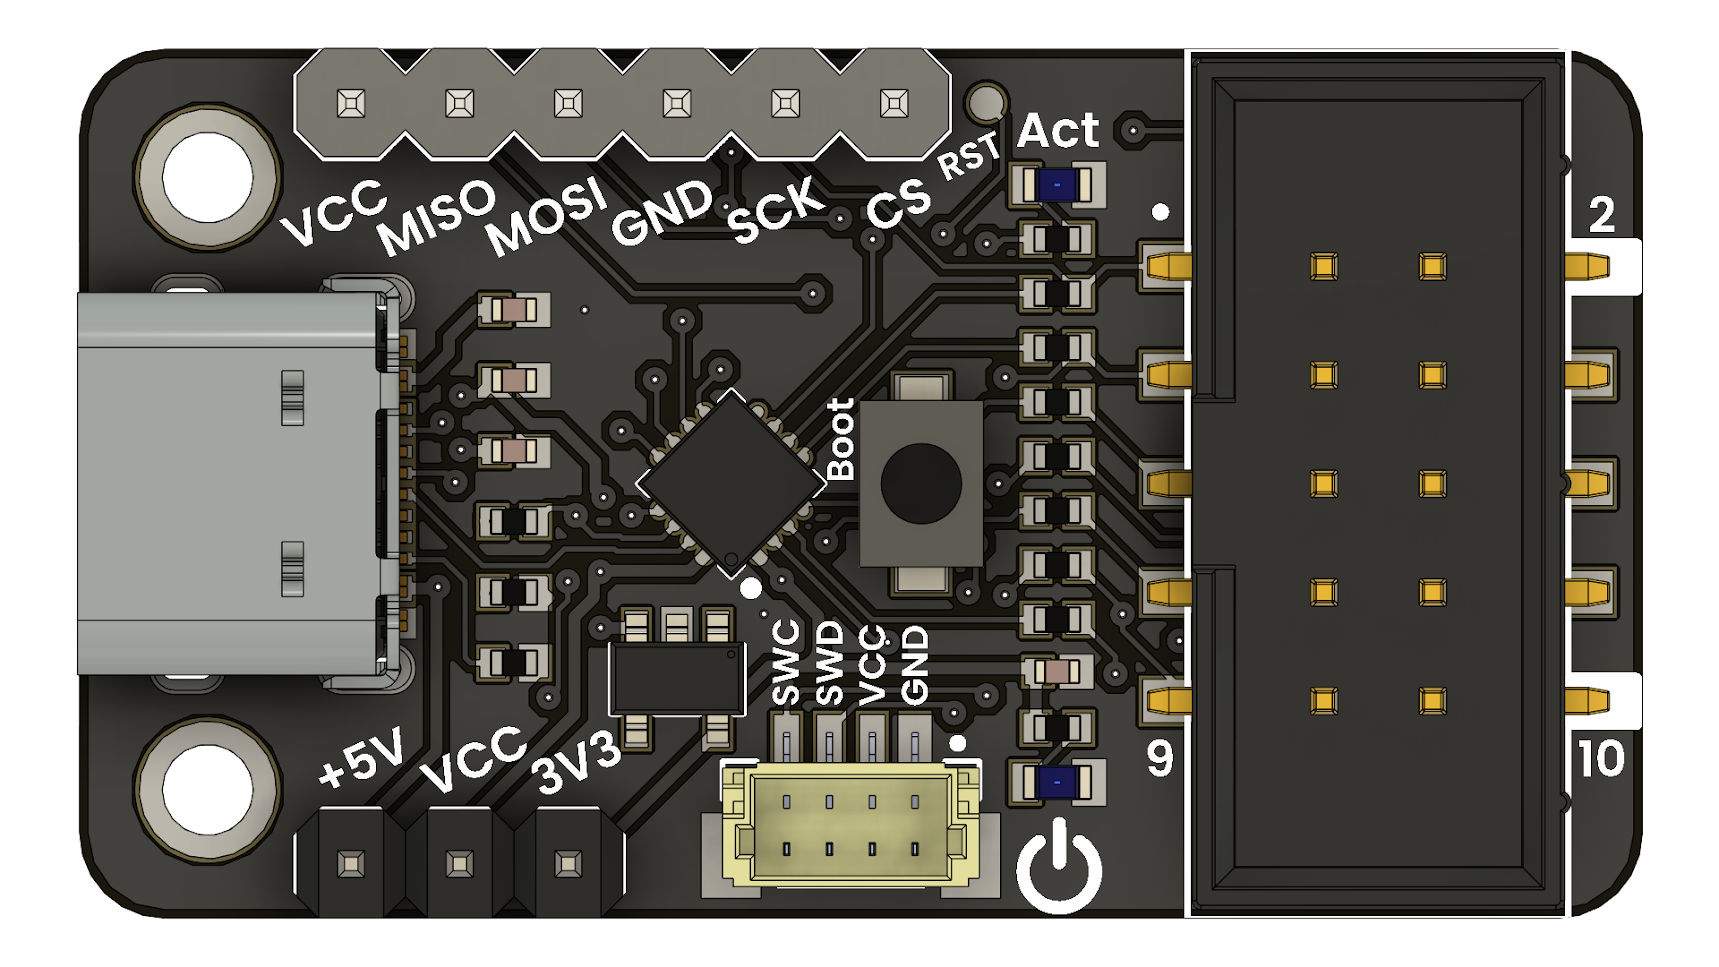
\includegraphics[height=4.5cm,keepaspectratio]{./images/product.png}
\end{minipage}

\vspace{1.0em}
\FloatBarrier % evita que la imagen flote sobre el siguiente bloque



% Secciones técnicas
\section*{Functional Description}
- USB Full-Speed interface (CDC or HID, depending on firmware)\\ 
- Programmable firmware profiles: AVR, CMSIS-DAP, and CPLD\\ 
- CH552G / CH552E microcontroller\\ 
- Selectable target voltage: 3.3V or 5V\\ 
- Bootloader mode for firmware flashing\\ 

\section*{Electrical Characteristics}
- The target voltage can be toggled between 3.3V and 5V using a physical switch.\\ 
- Programming interfaces include JTAG (TCK, TMS, TDI, TDO, nTRST) via a 2x5 1.27mm header, SWD (SWDIO, SWCLK) via a standard or JST connector, and SPI (MISO, MOSI, SCK, CS) via an inline header.\\ 
- A dedicated JST 1.0mm connector provides SWDIO, SWCLK, VCC, and GND for quick connections.\\ 

\section*{Features}
- Multiple firmware modes: AVR, ARM CMSIS-DAP, CPLD JTAG\\ 
- Standard USB HID/CDC communication\\ 
- Compatible with major programming tools (avrdude, OpenOCD, Quartus)\\ 
- Small footprint, easy to integrate into projects\\ 
- SDCC-compatible source code\\ 
- Support for Linux, and macOS\\ 



\section*{Applications}
- AVR programming via USBasp and UPDI\\ 
- ARM Cortex-M debugging via CMSIS-DAP (OpenOCD, PyOCD)\\ 
- JTAG programming for Intel/Altera MAX II CPLDs\\ 
- Universal compact programmer for educational kits\\ 
- Embedded development and prototyping\\ 

\vspace{1em}



\section*{Settings}

\subsection*{Interface Overview}
\rowcolors{2}{white}{rowalt}
\begin{tabularx}{\textwidth}{|c|c|>{\RaggedRight\arraybackslash}X|}
\hline
\rowcolor{headergray}
Interface & Signals / Pins & Typical Use \\
\hline
JTAG & TCK, TMS, TDI, TDO, nTRST & Full chip programming, in-circuit test, debug \\
SPI & MOSI, MISO, SCK, CS & Flash memory programming, peripheral data exchange \\
SWD & SWCLK, SWDIO & Cortex-M programming and debugging \\
JST Header & SWCLK, SWDIO, VCC, GND & Quick-connect to target board for SWD and power \\
\hline
\end{tabularx}


\subsection*{Supported Pins}
\rowcolors{2}{white}{rowalt}
\begin{tabularx}{\textwidth}{|c|c|>{\RaggedRight\arraybackslash}X|}
\hline
\rowcolor{headergray}
Symbol & I/O & Description \\
\hline
VCC & Input & Power supply (3.3V or 5V) \\
GND & - & Ground \\
BOOT & Input & Enter bootloader mode \\
P3.0 & I/O & General purpose (protocol-specific) \\
P3.1 & I/O & General purpose (protocol-specific) \\
P3.2 & Input & BOOT button \\
\hline
\end{tabularx}


\subsection*{Firmware Modes: AVR Programmer}
\rowcolors{2}{white}{rowalt}
\begin{tabularx}{\textwidth}{|c|>{\RaggedRight\arraybackslash}X|}
\hline
\rowcolor{headergray}
Feature & Description \\
\hline
Protocols & USBasp, Serial UPDI \\
Targets & ATmega, ATtiny, other AVR MCUs \\
Tools Supported & avrdude, PlatformIO \\
USB Mode & HID (USBasp), CDC (UPDI) \\
Voltage Output & 3.3V / 5V selectable \\
\hline
\end{tabularx}


\subsection*{Firmware Modes: CMSIS-DAP Debugger}
\rowcolors{2}{white}{rowalt}
\begin{tabularx}{\textwidth}{|c|>{\RaggedRight\arraybackslash}X|}
\hline
\rowcolor{headergray}
Feature & Description \\
\hline
Protocols & SWD, JTAG (CMSIS-DAP v1) \\
Targets & ARM Cortex-M (STM32, nRF52, SAMD, etc.) \\
Tools Supported & OpenOCD, PyOCD, Keil µVision, SEGGER \\
USB Mode & HID + optional CDC UART \\
Drivers & Native (Linux/macOS), Zadig (Windows) \\
\hline
\end{tabularx}


\subsection*{Firmware Modes: CPLD Programmer}
\rowcolors{2}{white}{rowalt}
\begin{tabularx}{\textwidth}{|c|>{\RaggedRight\arraybackslash}X|}
\hline
\rowcolor{headergray}
Feature & Description \\
\hline
Protocol & JTAG via USB-Blaster emulation \\
Targets & Intel/Altera MAX II (e.g., EPM240) \\
Tools Supported & Quartus Programmer \\
USB VID/PID & Safe: 0x16C0:0x05DC, Compatible: 0x09FB:0x6001 \\
Voltage Output & 3.3V / 5V selectable \\
\hline
\end{tabularx}






% Tabla principal
\section*{Pin \& Connector Layout}
\rowcolors{2}{white}{rowalt}
\begin{tabularx}{\textwidth}{|c|c|>{\RaggedRight\arraybackslash}X|}
\hline
\rowcolor{headergray}
Color & Signal Type & Description \\
\hline
Red & Power & Supply voltage (VCC) \\
Green & Ground & Common ground (GND) \\
Blue & SWD & SWDIO and SWCLK signals \\
Teal & SPI & SPI interface signals \\
Orange & JTAG & JTAG interface signals \\
Gray & Not Connected & Unused or reserved lines \\
Color & Signal Type & Description \\
\hline
\end{tabularx}


% Imágenes adicionales
\FloatBarrier
\newpage
\vspace*{3em}
\section*{Block Diagram}
\vspace{1em}
\begin{center}
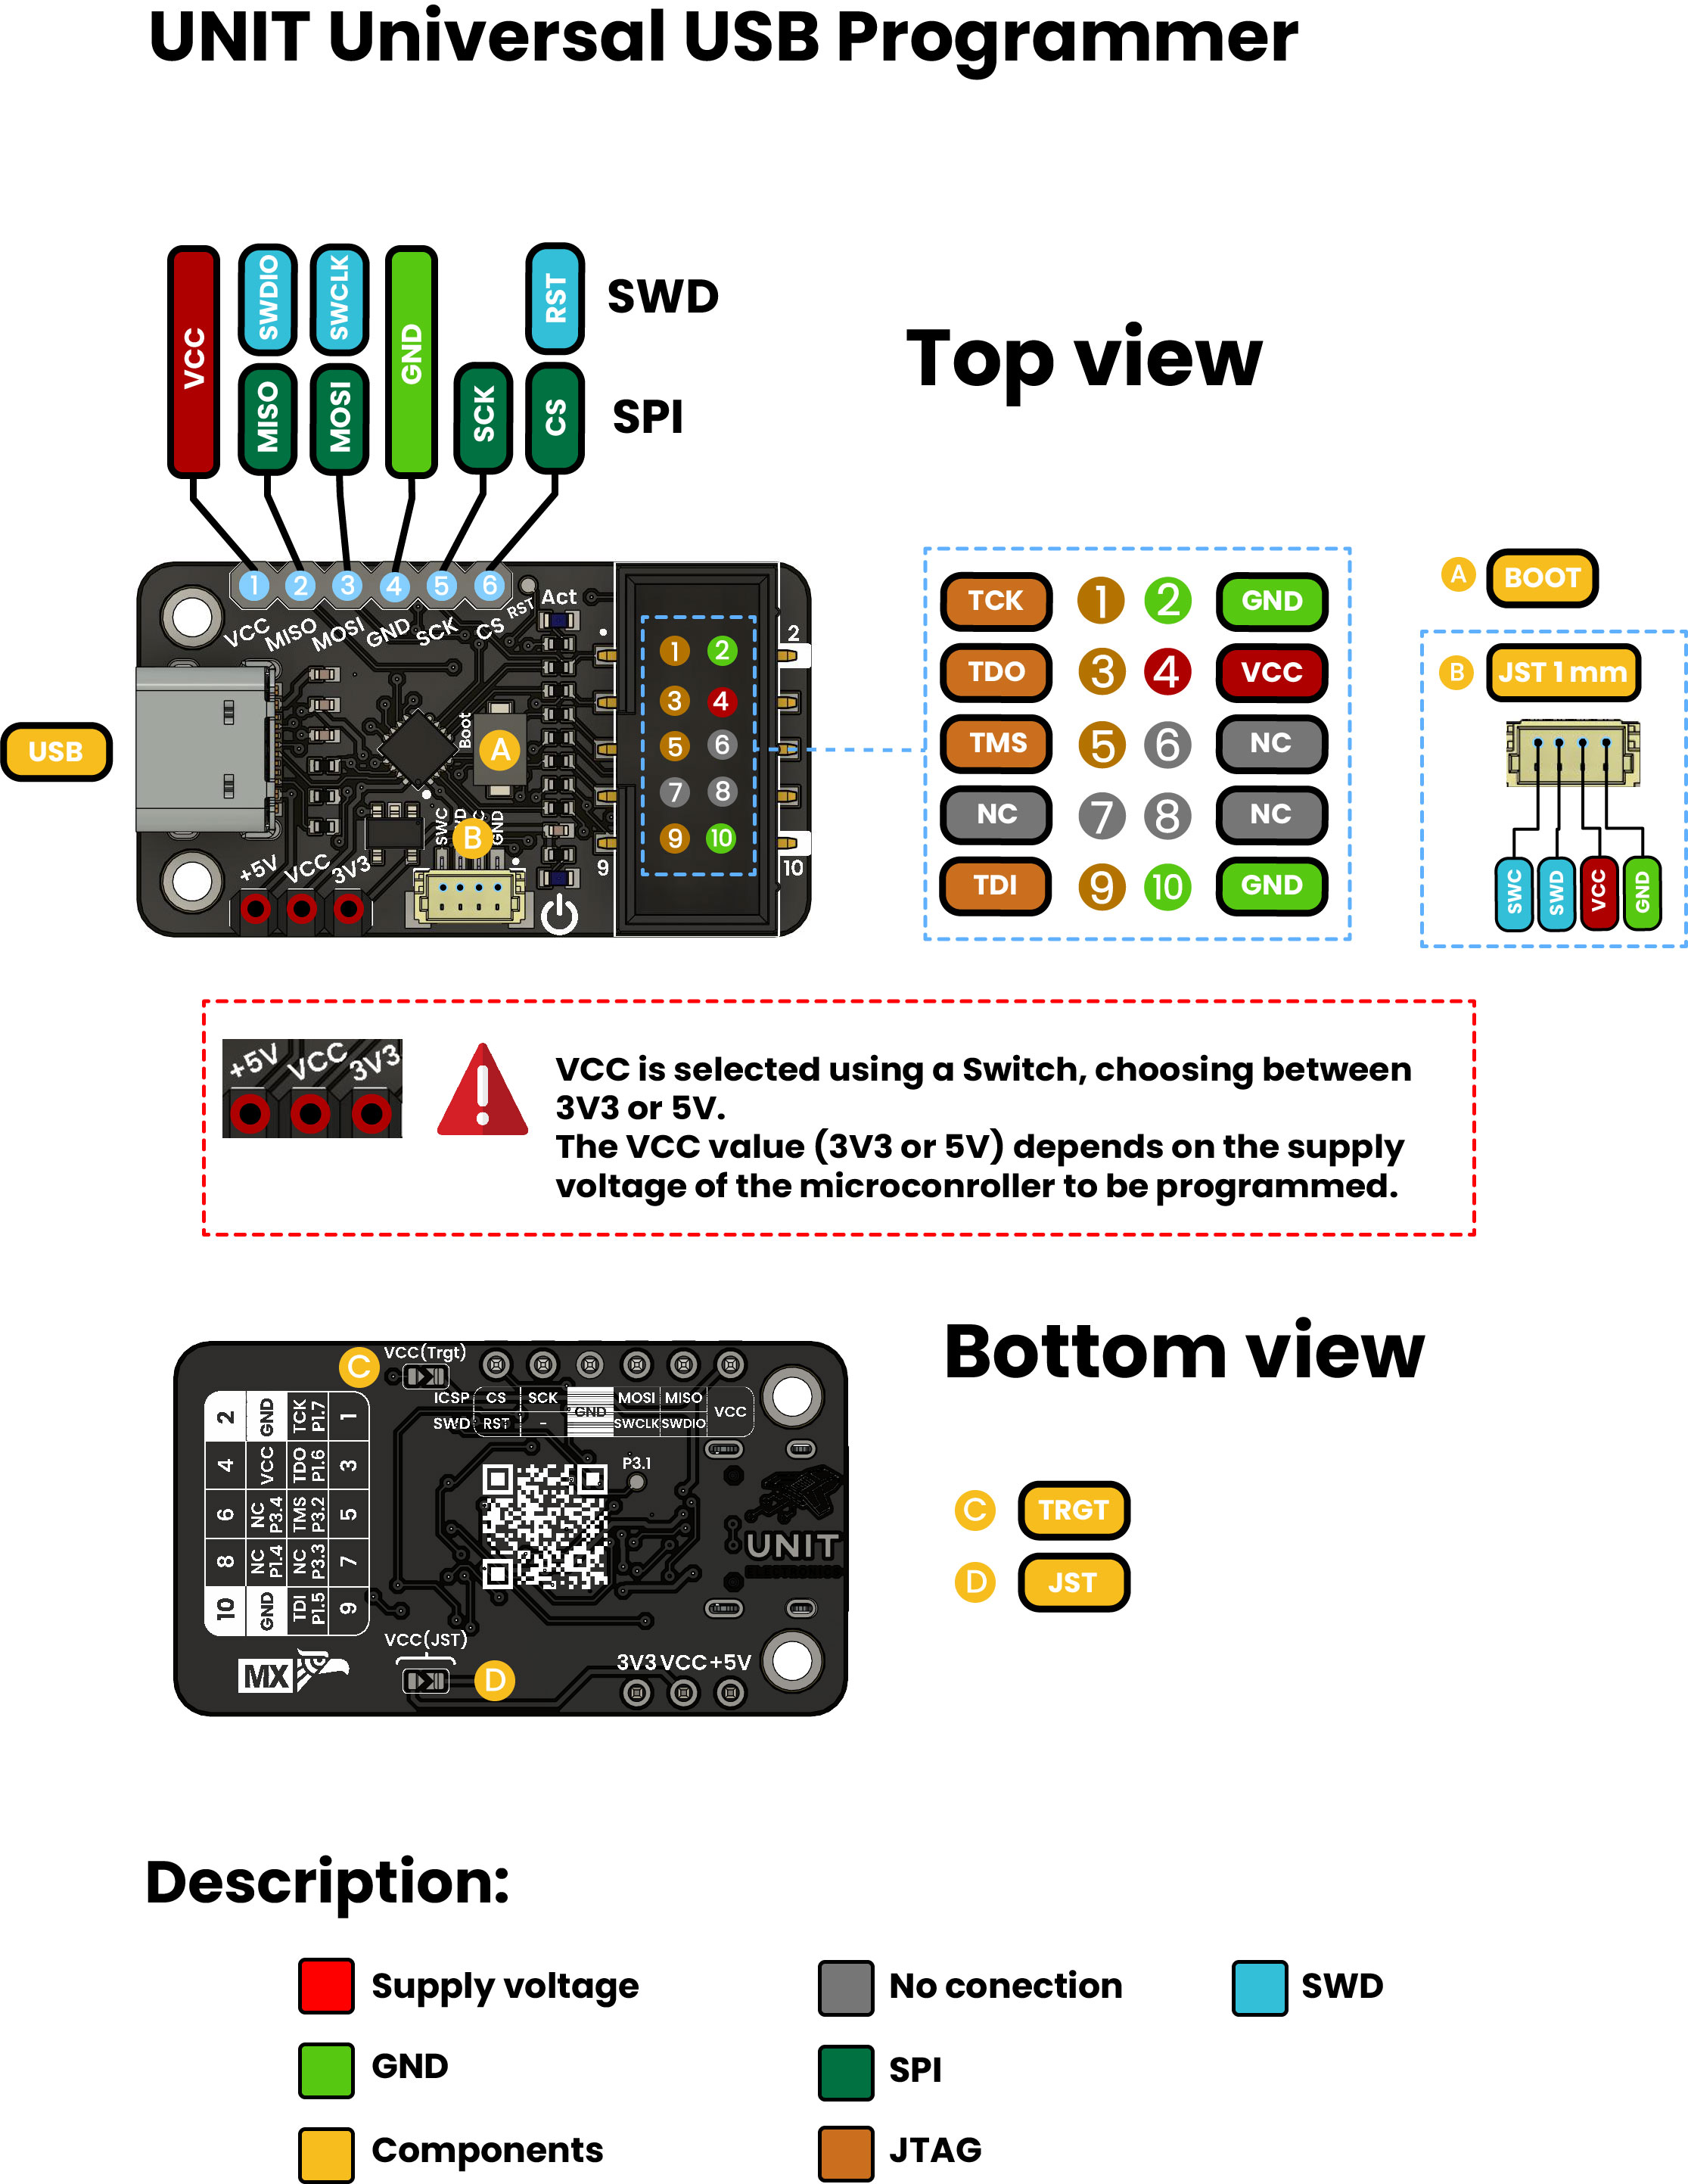
\includegraphics[width=0.95\textwidth,keepaspectratio]{images/function-diagram.jpg}
\end{center}
\newpage
\vspace*{3em}
\section*{Dimensions}
\vspace{1em}
\begin{center}
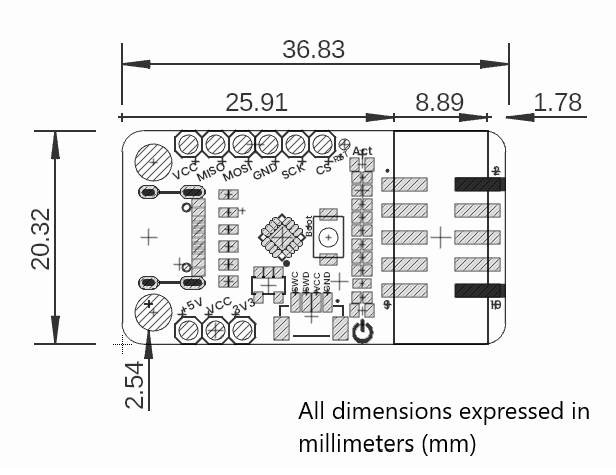
\includegraphics[width=0.95\textwidth,keepaspectratio]{images/dimensions.png}
\end{center}



% Uso
\section*{Usage}
\begin{itemize}
\item Arduino AVR
\item Raspberry Pi RP2040
\item STM32
\item NRF
\item PY32
\item MAX II
\end{itemize}

% Descargas
\section*{Downloads}
\begin{itemize}
\begin{itemize}
\item \href{docs/schematic.pdf}{Schematic PDF}
\item \href{https://github.com/UNIT-Electronics/MAX1704X_lib}{MAX1704X Library}
\end{itemize}
\end{itemize}

% Compra
\section*{Purchase}
\begin{itemize}
\item \href{https://www.uelectronics.com}{Buy from UNIT Electronics}
\end{itemize}

\end{document}
